\section{Introduction}
In this master thesis we will study how to implement an  electronic voting scheme application based on cryptography tools, most importantly the Publicly Verifiable Secret Sharing (PVSS) protocol and the multiparty computation protocol (MPC). The main paper for this protocol will be Berry Schoenmakers paper "A Simple Publicly Verifiable Secret Sharing Scheme and its Application to Electronic Voting" \cite{Schoenmakers1999}. \\\\
\noindent
The PVSS protocol is based on secret sharing. Secret sharing is way
of distributing a secret among multiple parties, where each party gets a subset of the secret. The individuel party member cannot extract any information about the secret from his subset alone, but if enough parties pulls there shares together, they will be able to recontruct the secret. More technically the idea is to hide a secret inside of a polynomial so that given certain partial information of the polynomial we can recover the secret that was hidden in it.\\\\
\noindent
The MPC protocol is a protocol which uses secret sharing and allows several parties to compute some function on some private inputs, in such a way that they learn the result but not the inputs from the other players. MPC is not using conventional methods, where some commonly trusted party, could gather sensitive information. In the left image of figure \ref{fig:MPC_Overview} it shows a judge who all participants trust to give their secret inputs. The trusted party can then compute the outcome of the process, for instance the sum of all inputs, and reveal the output. The right figure is how an equivalent MPC would work. Here there is no trusted party, but by using multiparty computation they can still achieve the same level of secrecy, but without having to trust someone.

\begin{figure}[H]
    \centering
    \makebox[\textwidth]{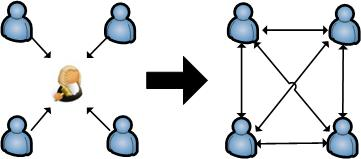
\includegraphics[scale=0.9]{MPC_Overview.jpg}}
    \caption{Multiparty computation overview}
    \label{fig:MPC_Overview}
\end{figure} 

\noindent
This leads to a core observation namely that without a trusted party the ability to validate the input the MPC protocol relies on the participants honesty. 
The PVSS protocol used in this thesis proposes a solution to this problem. The idea is that not only can the participants verify their own shares, but that anybody can verify the correctness of the transmitted data.